\documentclass{article}

% NeurIPS 2022 style (course template). natbib is loaded by neurips_2022 -> \citep/\citet work.
\usepackage[final]{neurips_2022}

\usepackage[utf8]{inputenc} % allow utf-8 input
\usepackage[T1]{fontenc}    % use 8-bit T1 fonts
\usepackage{hyperref}       % hyperlinks
\usepackage{url}            % simple URL typesetting
\usepackage{booktabs}       % professional-quality tables
\usepackage{amsfonts}       % blackboard math symbols
\usepackage{amssymb}
\usepackage{amsmath}
\usepackage{nicefrac}       % compact symbols for 1/2, etc.
\usepackage{microtype}      % microtypography
\usepackage{xcolor}
\usepackage{graphicx}       % figures (\includegraphics)
\usepackage{tikz}           % architecture schematic
\usetikzlibrary{arrows.meta,positioning,fit,backgrounds}

% pandoc emits \tightlist inside compact lists; define it (we use our own preamble, not pandoc's template).
\providecommand{\tightlist}{\setlength{\itemsep}{0pt}\setlength{\parskip}{0pt}}

\title{What Is the Accuracy Made Of? Auditing a Competitive\\ AI-Generated Image Detector with a Concept Bottleneck}

% TODO (H-1): replace the bracketed placeholders with the real author name and email before submission.
% (email wrapped in \texttt so the preceding \\ does not parse "[...]" as an optional length argument.)
\author{%
  [Your Name] \\
  Shanghai Jiao Tong University \\
  \texttt{[email@example.com]}
}

\begin{document}

\maketitle

\begin{abstract}
AI-generated image detection has advanced to the point where, on the standard GenImage benchmark, recent detectors report near-saturated cross-generator accuracy; our own deliberately conventional, single-GPU detector reaches 99.67\% mean accuracy on held-out GenImage generators. A saturated benchmark, however, leaves open what such numbers are made of: a high score can reflect either the detection of generative traces or the exploitation of incidental dataset artifacts. We study this question from inside the model. Our detector---a dual-stream backbone with a six-channel concept bottleneck and a linear head---has one essential property: the prediction passes through six separately-testable evidence channels and nothing else. We use this bottleneck not as an interpretability device but as an audit instrument, measuring each channel's contribution causally, by ablation and counterfactual, rather than reading it from weights or post-hoc narration. The audit shows that the detector's decision turns on a frequency/compression cue pair (jpeg-quant and freq-radial, $r{=}{-}0.80$)---localized by intervention; the carrier label shifts across seeds, but the pair-level reliance is stable, a finding weight inspection alone would miss---and that this reliance persists even after Grommelt-style JPEG debiasing neutralizes the obvious container cue (replicated across three seeds, with seed-dependent strength), so the compression axis is not reducible to the image-format label---though we cannot exclude a residual JPEG re-encoding signature as the surviving cue. The headline accuracy is thus partly confound-inflated: it drops substantially on a container-mismatched benchmark, though multi-generator training still buys genuine partial cross-architecture generalization. We extend prior dataset-level analyses of GenImage confounds to a model-internal account---where the reliance lives, how large it is, and whether it survives debiasing---and argue that a concept bottleneck's value lies in being a testability surface. A no-bottleneck baseline matches this accuracy (99.60\% OOD) and is equally confound-susceptible, confirming the bottleneck adds audit visibility at zero accuracy cost. We report competitive, not state-of-the-art, detection.

\end{abstract}

\section{Introduction}

Generative image models have advanced to the point where their outputs are, for many categories of content, perceptually indistinguishable from real photographs. Generative adversarial networks \citep{brock2018biggan} established high-fidelity synthesis, and latent-diffusion and text-to-image systems \citep{rombach2022ldm, dhariwal2021adm, nichol2022glide} have since made photorealistic generation cheap, controllable, and ubiquitous. The resulting flood of synthetic imagery poses concrete risks for misinformation, fraud, and the integrity of visual evidence, and has made AI-generated image detection (AGID) a central problem in media forensics. On the field's dominant benchmark, GenImage \citep{zhu2023genimage}, detection accuracy has effectively saturated: methods spanning spatial-domain classifiers \citep{wang2020cnngenerated}, neighborhood-pixel-relationship residuals \citep{tan2024npr}, bit-plane representations \citep{wang2025lota}, and multimodal large-language-model reasoning \citep{zhou2025aigiholmes} now routinely report cross-generator accuracies above 98\%. By the usual reading, AGID is close to solved.

A saturated benchmark, however, raises a question the accuracy figure alone cannot settle. A detector earns a high number whenever its inputs contain \emph{any} feature that separates the \emph{real} and \emph{AI} partitions of the dataset---whether that feature is a generative trace intrinsic to the synthesis process, or an incidental artifact of how the dataset was assembled. The two are indistinguishable from the loss curve, yet only the former is what we intend to measure. The pressing question behind the leaderboard is therefore not \emph{how accurate is the detector?} but \emph{what is the accuracy made of?}

Two obstacles stand between the field and an answer. The first is that interpretability in AGID is generally \emph{asserted} rather than \emph{causally tested}. Concept-bottleneck models \citep{koh2020concept} and, more recently, MLLM-based detectors such as AIGI-Holmes \citep{zhou2025aigiholmes} attach human-legible explanations to their predictions---named concepts, or natural-language rationales describing anatomical errors and physical-law violations. But an explanation produced \emph{alongside} a decision is not necessarily the \emph{cause} of that decision; the concept-bottleneck literature has itself repeatedly documented that learned concepts can be unfaithful, leaky, or unused \citep{margeloiu2021concept, mahinpei2021promises, havasi2022addressing}. In AIGI-Holmes the rationale is generated by a separate language module whose fidelity to the visual detector's actual computation is never verified. Interpretation, in short, is offered but not intervened upon.

The second obstacle is that the \emph{measurement validity} of the benchmark is under-examined at the level of the model. \citet{grommelt2024fakejpeg} recently established that GenImage and comparable datasets carry systematic biases---most notably a JPEG-compression confound (real images are stored as JPEG, many synthetic images as lossless PNG) and an image-size confound---and that black-box detectors learn to exploit them: re-encoding every image to a uniform JPEG quality materially changes cross-generator performance. This is a crucial dataset-level diagnosis. But because it is obtained with black-box classifiers, it establishes only \emph{that} a confound exists and \emph{that} detectors are sensitive to it; it does not reveal \emph{how} an individual model distributes its decision across such cues, \emph{how much} of a given detector's competence rests on the confound rather than on generative traces, or \emph{whether} that competence would survive removal of the confound. These are model-internal questions, and answering them requires a model-internal instrument.

The field thus presents a dilemma: strong but opaque detectors on one side, and interpretable-by-assertion detectors whose explanations are seldom tested on the other. What is missing---and what this paper supplies---is an architecture-level audit mechanism that can intervene on separately-testable evidence channels inside a competitive detector: a model whose prediction provably routes through a small set of named cues, each of which can be individually ablated, swapped, and re-measured.

We present \textbf{CBNet-AGID}, a \emph{deliberately conventional}, single-GPU detector assembled from standard components: an ImageNet-pretrained ResNet-50 stream, a neighborhood-pixel-relationship residual stream \citep{tan2024npr}, a six-channel concept-bottleneck layer, and a linear classifier with no skip connection from features to output. We are explicit about what we do and do not claim for this architecture. We do \textbf{not} claim its six channels are intrinsically interpretable or individually faithful: their semantic identities are induced by weak heuristic supervision, not enforced by the architecture---and one of our central findings is precisely that these identities cannot be taken at face value. What the architecture \emph{does} guarantee is narrower and, for our purpose, more valuable: that the prediction is a linear function of the six channel activations alone, with no bypass path. This turns the bottleneck into an \textbf{audit instrument}---a surface on which each evidence channel's contribution to the decision can be measured \emph{causally}, by zeroing or counterfactually swapping it, rather than inferred from correlations or from the model's own narration. We deliberately keep the detector conventional so that what the audit finds reflects the behaviour of standard strong detectors rather than an idiosyncratic architecture.

Applying this instrument to a detector trained jointly on four GenImage generators yields a sharp picture. A compression-axis pair of channels---jpeg-quant and freq-radial, correlated at $r{=}{-}0.80$---dominates the decision: ablating both collapses balanced accuracy to chance on every generator, and ablating either one alone costs 17--50\,pp depending on the random seed (\S{}4.3a). A causal counterfactual confirms these are the channels the decision actually turns on, while the bottleneck's remaining four channels carry little \emph{independent} signal. The linear-head weights do \emph{not} reveal this---which of the two correlated channels the head names as the primary carrier shifts across seeds, and the magnitudes are far more evenly distributed than the ablation numbers---so only intervention exposes the dependency, underscoring that weight inspection is an unreliable proxy for functional reliance and that causal ablation is the appropriate test. Crucially, this reliance is not merely the obvious container cue. When we retrain the identical architecture on a Grommelt-style debiased corpus---every image re-encoded to a uniform JPEG quality of 96, neutralizing the PNG-versus-JPEG container gap at the data level---the model still routes its largest single-channel reliance through the same compression axis in every seed, though the magnitude is seed-dependent (a dominant single-channel cost of 8--48 points across three seeds; \S{}4.3c). The channel is therefore \emph{not reducible} to the trivial container label; whether it captures genuine generative-pipeline traces or residual compression-history statistics that survive uniform re-encoding is a question our experiments cannot fully resolve, and we are careful not to overstate it.

Finally, the audit lets us read the headline number honestly. On held-out GenImage generators the detector reaches 99.67\% mean accuracy---competitive with the strongest reported single-GPU methods. But that figure is partly a property of the benchmark rather than of the detector: evaluated on ForenSynths \citep{wang2020cnngenerated}, a cross-architecture benchmark drawn from different real and synthetic sources that do not share GenImage's container statistics, the same model attains 73.65\%. The 26-point drop indicates that a substantial share of the GenImage number does not transfer; yet 73.65\% is also well above an otherwise-identical single-generator model, which is barely above chance---indicating that multi-generator training buys \emph{genuine} partial cross-architecture generalization. The honest summary is neither ``the detector merely exploits a confound'' nor ``the detector robustly generalizes,'' but both at once---partial confound inflation alongside genuine partial generalization---and we attribute neither all nor none of the cross-benchmark gap to the confound, since it is entangled with a real GAN-versus-diffusion distribution shift.

These observations organize the paper around two research questions:

\begin{itemize}
\tightlist
\item
  \textbf{RQ1 (Detection).} Can a deliberately standard, single-GPU concept-bottleneck detector attain competitive cross-generator accuracy on GenImage?
\item
  \textbf{RQ2 (Audit).} What does that accuracy rest on---which separately-testable evidence channels does the detector rely upon, how much does each contribute under causal intervention, does that reliance survive dataset-level debiasing, and how much of the headline GenImage number is artifact-inflated versus genuinely generalizing?
\end{itemize}

Our contributions are as follows. \textbf{(1)} We repurpose a concept bottleneck as an \emph{architecture-level audit instrument} for AGID---separately-testable evidence channels with a no-bypass guarantee that makes per-channel faithfulness \emph{causally testable} rather than assumed. \textbf{(2)} Using it, we give a \emph{model-internal localization} of the GenImage confound, showing that a competitive detector's decision turns causally on a compression-axis channel pair (jpeg-quant and freq-radial, $r{=}{-}0.80$)---ablating the pair collapses accuracy to chance, with the dominant carrier label shifting across random seeds while the pair-level reliance remains stable. \textbf{(3)} We quantify this reliance by \emph{causal intervention}---single-channel ablation and counterfactual swaps---and show that the linear weights would have mis-attributed it (the rank-1 weight shifts across seeds). \textbf{(4)} We show the reliance \emph{persists under Grommelt-style debiasing} (a persistence result we label Outcome C, replicated across three random seeds with seed-dependent strength), extending \citet{grommelt2024fakejpeg}'s dataset-level diagnosis to a model-internal one, and we bound how much of the benchmark number is confound-inflated through a cross-architecture (ForenSynths) comparison. The competitive detector itself is not our headline claim; it is the \emph{subject} of the audit. Throughout, we are explicit about scope: we report \emph{competitive}, not state-of-the-art, detection---our joint multi-generator training protocol differs from the single-generator protocols of the methods we tabulate, as detailed in \S{}4.1---and we frame our generalization findings as partial in both directions.

\section{Related Work}

\textbf{Generalizable AGID detectors.} The modern AGID literature is organized around one goal: a detector trained on one or a few generators that generalizes to unseen ones. Early work showed that a plain CNN trained on ProGAN images transfers surprisingly well across GAN families \citep{wang2020cnngenerated}, and subsequent methods improved cross-generator transfer through frequency-domain cues \citep{frank2020dctgan, durall2020watch, tan2024freqnet}, neighborhood-pixel-relationship residuals \citep{tan2024npr}, bit-plane decompositions \citep{wang2025lota}, reconstruction error from diffusion inversion \citep{wang2023dire}, and features from frozen vision--language backbones \citep{ojha2023universal}. On GenImage \citep{zhu2023genimage}, the de-facto standard benchmark, the strongest of these report cross-generator accuracies in the high-90s, and the field increasingly treats GenImage performance as near-saturated. These detectors are, however, black boxes: each exposes a single decision score with no internal, separately-testable account of which evidence a prediction rests on. And as a matter of measurement, these near-saturated GenImage numbers may reflect not only generative-trace detection but also dataset shortcuts \citep{geirhos2020shortcut}---a concern raised specifically for AGID by \citet{grommelt2024fakejpeg} and one we test model-internally in our experiments. The accuracy is established; what the accuracy rests on is not.

\textbf{Interpretable detection and concept bottlenecks.} A parallel line of work seeks detectors that \emph{explain} their decisions. Concept-bottleneck models route prediction through a layer of human-named concepts \citep{koh2020concept}, and explainable AGID has lately been pursued most visibly through multimodal LLMs: AIGI-Holmes \citep{zhou2025aigiholmes}, for instance, pairs a visual detector with a tuned language model that narrates anatomical, physical, and common-sense anomalies, while related systems generate chain-of-thought or grounded rationales \citep{huang2025thinkfake, tan2025forenx, ji2025grounded}. The difficulty is that such explanations are validated, if at all, by their plausibility to a human reader rather than by their causal role in the decision. This is not a hypothetical worry: the concept-bottleneck literature has documented that learned concepts may fail to mean what their labels say---they can be unfaithful to the underlying computation \citep{margeloiu2021concept}, leak information through their soft activations \citep{havasi2022addressing}, or simply go unused as intended \citep{mahinpei2021promises}. For MLLM rationales the problem is sharper still, because the narration is produced by a module structurally distinct from the detector and is, by construction, un-intervenable: one cannot ablate a sentence and re-measure the decision. AIGI-Holmes is thus the natural foil for our work---interpretability at its most expressive and least falsifiable. We take the opposite stance. We do not claim our concepts are interpretable by construction; we claim only that the bottleneck makes per-channel reliance \emph{causally testable}, and we carry out that test---single-channel ablation and concept-sensitivity probes in the spirit of \citet{kim2018tcav} and insertion/deletion analysis \citep{petsiuk2018rise}---rather than assert its outcome.

\textbf{Dataset confounds in AGID benchmarks.} Closest to our diagnostic aim is recent work on benchmark biases. \citet{grommelt2024fakejpeg} show that GenImage and similar corpora conflate ``generated-ness'' with incidental acquisition artifacts---chiefly a JPEG-compression gap (real images stored as JPEG, many synthetic images as lossless PNG) and an image-size gap---and that conventional black-box detectors learn these shortcuts, so that debiasing the data by uniform re-encoding shifts cross-generator performance. We build directly on this finding and credit it as the origin of the confound diagnosis: we do not claim to \emph{discover} that GenImage is confounded. Our contribution is complementary and orthogonal in vantage point. Grommelt's analysis is conducted from the outside, with black-box classifiers, and establishes the confound at the level of the \emph{dataset}. We provide the corresponding account at the level of the \emph{model}: using the bottleneck as an instrument, we localize the confound to a specific evidence channel, quantify by causal intervention how much of a competitive detector's accuracy flows through it, and ask---by retraining on Grommelt-style debiased data---whether that reliance is removed or merely relocated.

\textbf{The gap.} Taken together, the field offers strong but opaque detectors, interpretable-by-assertion detectors whose explanations are not causally tested, and a dataset-level diagnosis of confounding obtained without looking inside any model. What no prior work provides is an architecture-level audit mechanism that can intervene on separately-testable evidence channels within a competitive detector---turning the question ``what is the accuracy made of?'' from a matter of inference into one of measurement. That mechanism, and the model-internal account of GenImage's confound it yields, is the subject of this paper.

\section{Method}

\subsection{Overview}

We treat AI-generated image detection as binary classification: given an RGB image \(I\), predict \(y\in\{0,1\}\) (\(0\) = real, \(1\) = AI-generated). Our detector, CBNet-AGID, is a three-stage pipeline (a dual-stream backbone \(f_\theta\), a concept-bottleneck layer \(C_\phi\) of \(K{=}6\) channels, and a linear classifier \(\mathbf{w}\)) arranged so that every prediction is, by construction, a linear function of six separately-testable evidence channels and nothing else. The design is \emph{deliberately conventional}: each component is a standard, off-the-shelf building block, and we make \textbf{no claim of architectural novelty}. Its purpose is not raw performance but \textbf{auditability}---the no-skip bottleneck of \S{}3.3 is what licenses the causal intervention analysis (\S{}3.7) that constitutes this paper's contribution. The model has \ensuremath{\sim}38M parameters and trains and runs on a single 8GB consumer GPU; \autoref{fig:arch} shows the full pipeline.

% CBNet-AGID architecture schematic (TikZ, vector). Mirrors Method section 3.1-3.3.
% Key message: the linear classifier sees ONLY the 6-channel bottleneck c -- no skip
% path from the backbone f_theta. The compression-pair channels are shaded to match
% the channel-reliance figure.
\begin{figure}[t]
  \centering
  \resizebox{\textwidth}{!}{%
  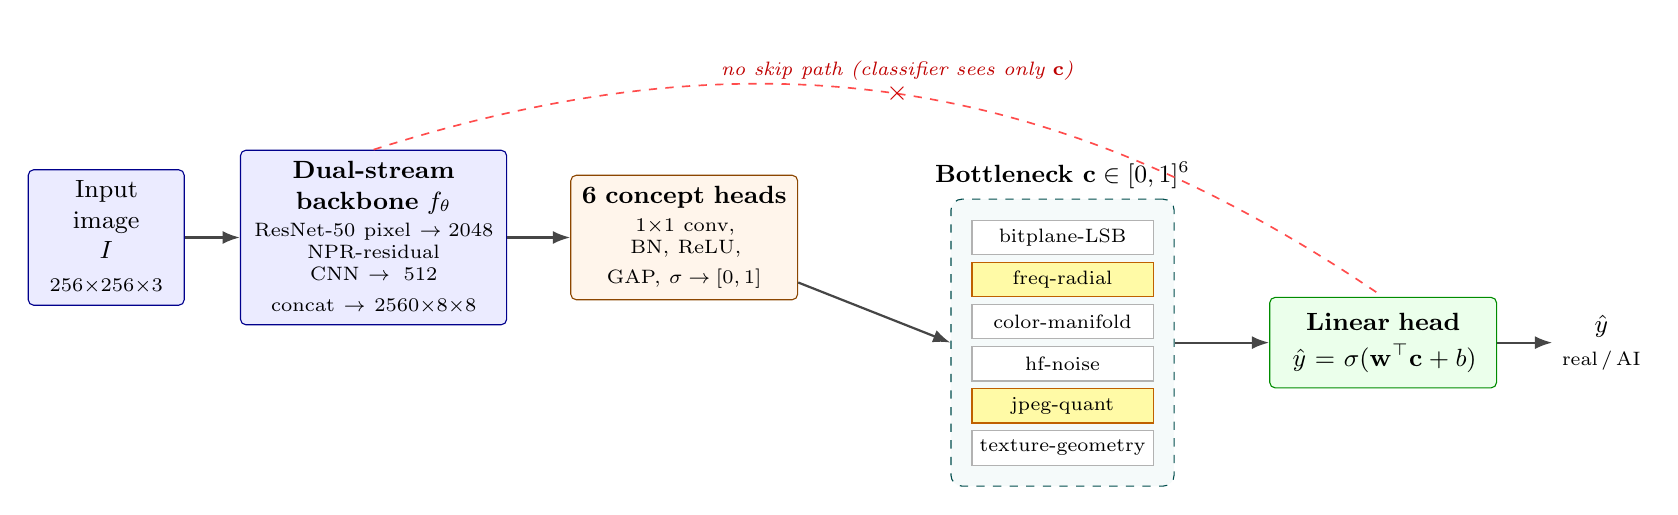
\begin{tikzpicture}[
    font=\small,
    >={Latex[length=2.2mm]},
    box/.style={draw=#1!55!black, fill=#1!8, rounded corners=2pt, align=center,
                inner sep=4pt, minimum height=1.15cm},
    cell/.style={draw=gray!60, fill=white, minimum width=2.3cm, minimum height=0.44cm,
                 inner sep=1pt, font=\scriptsize, align=center},
    cellhi/.style={cell, fill=yellow!35, draw=orange!75!black},
    flow/.style={->, thick, gray!55!black},
  ]
    % --- main pipeline ---------------------------------------------------
    \node[box=blue, text width=1.7cm] (img)
      {Input image\\$I$\\[1pt]\scriptsize$256{\times}256{\times}3$};
    \node[box=blue, right=7mm of img, text width=3.1cm] (bb)
      {\textbf{Dual-stream backbone} $f_\theta$\\[2pt]
       \scriptsize ResNet-50 pixel $\to 2048$\\
       \scriptsize NPR-residual CNN $\to 512$\\
       \scriptsize concat $\to 2560{\times}8{\times}8$};
    \node[box=orange, right=8mm of bb, text width=2.6cm] (heads)
      {\textbf{6 concept heads}\\[2pt]
       \scriptsize $1{\times}1$ conv, BN, ReLU,\\
       \scriptsize GAP, $\sigma\!\to\![0,1]$};

    % --- bottleneck: six stacked channel cells (compression pair shaded) --
    \node[cell, right=22mm of heads] (c1) {bitplane-LSB};
    \node[cellhi, below=0.8mm of c1]  (c2) {freq-radial};
    \node[cell,   below=0.8mm of c2]  (c3) {color-manifold};
    \node[cell,   below=0.8mm of c3]  (c4) {hf-noise};
    \node[cellhi, below=0.8mm of c4]  (c5) {jpeg-quant};
    \node[cell,   below=0.8mm of c5]  (c6) {texture-geometry};

    \begin{scope}[on background layer]
      \node[draw=teal!60!black, dashed, rounded corners, fill=teal!4,
            fit=(c1)(c6), inner sep=2.6mm,
            label={[font=\small\bfseries]above:{Bottleneck $\mathbf{c}\in[0,1]^6$}}] (bn) {};
    \end{scope}

    % --- linear head + output -------------------------------------------
    \node[box=green, right=12mm of bn, text width=2.6cm] (lin)
      {\textbf{Linear head}\\[2pt]$\hat{y}=\sigma(\mathbf{w}^\top\mathbf{c}+b)$};
    \node[right=7mm of lin, align=center] (out)
      {$\hat{y}$\\[1pt]\scriptsize real\,/\,AI};

    % --- arrows ----------------------------------------------------------
    \draw[flow] (img) -- (bb);
    \draw[flow] (bb) -- (heads);
    \draw[flow] (heads) -- (bn.west);
    \draw[flow] (bn.east) -- (lin);
    \draw[flow] (lin) -- (out);

    % --- "no skip" forbidden bypass -------------------------------------
    \draw[dashed, red!70, line width=0.6pt]
      (bb.north) to[bend left=26] coordinate[pos=0.5](mid) (lin.north);
    \node[red!80!black, font=\bfseries] at (mid) {$\times$};
    \node[red!75!black, font=\scriptsize\itshape, above=0.5mm of mid]
      {no skip path (classifier sees only $\mathbf{c}$)};
  \end{tikzpicture}}
  \caption{\textbf{CBNet-AGID: a deliberately conventional detector with an audit
    surface.} A dual-stream backbone (ImageNet Res-50 pixel stream + NPR-residual
    signal stream) is concatenated and mapped by six architecturally identical heads to a
    six-channel concept bottleneck $\mathbf{c}\in[0,1]^6$. The linear classifier reads
    \emph{only} $\mathbf{c}$: there is no skip connection from $f_\theta$ to the output
    (red, forbidden), so every prediction is a linear function of the six
    separately-testable evidence channels and nothing else. This no-bypass property is what
    makes each channel's contribution \emph{causally} measurable by zeroing or swapping it
    (\S{}3.7). Shaded cells mark the correlated compression pair
    (\texttt{freq-radial}, \texttt{jpeg-quant}; $r{=}{-}0.80$) that the audit finds
    load-bearing (\autoref{fig:reliance}).}
  \label{fig:arch}
\end{figure}


\subsection{Dual-stream backbone}

The backbone fuses two parallel streams operating on the same input. The \textbf{pixel stream} is a standard ImageNet-pretrained ResNet-50 \citep{he2016resnet}, producing a \(2048\times8\times8\) feature map for a \(256\times256\) input. The \textbf{signal stream} operates on the neighborhood-pixel-relationship residual of \citet{tan2024npr}, \(r(I)=I-\mathcal{U}(\mathcal{D}(I))\), where \(\mathcal{D},\mathcal{U}\) are nearest-neighbor down- and up-sampling by a factor of two; a lightweight five-layer strided CNN (\ensuremath{\sim}3M parameters) maps \(r(I)\) to a \(512\times8\times8\) map. The two are concatenated channel-wise into \(f_\theta(I)\in\mathbb{R}^{2560\times8\times8}\). Both streams are off-the-shelf; their pairing is an engineering convenience for capturing low- and high-level cues, not a contribution.

\subsection{Concept-bottleneck layer: the audit surface}

The bottleneck \(C_\phi\) comprises \(K{=}6\) \textbf{architecturally identical} heads. Each head \(h_{\phi_k}\) applies a \(1\times1\) convolution (\(2560\to640\)), batch-norm, ReLU, and a second \(1\times1\) convolution to a single spatial map; the scalar channel activation is \(c_k(I)=\sigma\big(\mathrm{GAP}(h_{\phi_k}(f_\theta(I)))\big)\in[0,1]\), with the pre-pooling map retained as a heatmap for localization. The channel vector \(\mathbf{c}(I)=[c_1,\dots,c_6]\) feeds a linear classifier: \[\hat{y}(I)=\sigma\big(\mathbf{w}^\top\mathbf{c}(I)+b\big).\] Two properties are essential. \textbf{(i) No skip connection:} the classifier sees \emph{only} \(\mathbf{c}(I)\)---never \(f_\theta(I)\)---so the six scalars are the sole information path from image to decision. This is the load-bearing property of the architecture: it is what makes a channel's functional role \emph{causally} measurable by perturbing \(c_k\). \textbf{(ii) Linear head:} each channel's contribution to the logit is exactly \(w_k c_k\), fully decomposable.

Crucially, because the six heads are \emph{identical in form}, a channel's identity is conferred only by the weak supervision that shapes it (\S{}3.4), not by any architectural commitment. We therefore refer to the \(c_k\) as \textbf{separately-testable evidence channels} rather than interpretable concepts: the bottleneck guarantees that the decision passes through them and that each can be individually intervened upon, but it does \textbf{not} guarantee that channel \(k\) means what its name suggests. Whether it does is an empirical question we settle by intervention (\S{}3.7), not by assertion---a stance that distinguishes our use of the concept-bottleneck construction \citep{koh2020concept} from interpretability-by-design claims.

\subsection{Evidence channels and weak supervision}

No concept-annotated AGID dataset exists, so we supervise each channel with a cheap, non-parametric image-statistic heuristic that produces a soft label \(\tilde{c}_k(I)\in[0,1]\); heads are trained to match these labels (\S{}3.5). The six channels are: \textbf{bitplane-LSB} (horizontal autocorrelation of the grayscale least-significant-bit plane); \textbf{freq-radial} (slope of the log--log radial power spectrum); \textbf{color-manifold} (KL divergence of the image's RGB histogram from a shared real-image color prior); \textbf{hf-noise} (variance of the Laplacian); \textbf{jpeg-quant} (variance of DCT-coefficient residuals after re-quantization---a JPEG-quantization-trace signal); and \textbf{texture-geometry} (decoupling of per-patch edge density from per-patch intensity variance). The labels require no human annotation. We re-emphasize that these heuristics define \emph{training targets}, not guaranteed semantics: the trained channel may track its heuristic faithfully or may drift under the task objective, which is precisely what the audit measures.

\subsection{Training objective}

We minimize a weighted sum of four terms, \[L = L_{\text{task}} + \lambda_c L_{\text{concept}} + \lambda_p L_{\text{pair}} + \lambda_s L_{\text{sparsity}},\qquad (\lambda_c,\lambda_p,\lambda_s)=(0.5,\,0.2,\,0.05),\] where \(L_{\text{task}}\) is the binary cross-entropy of \(\hat{y}\) against \(y\); \(L_{\text{concept}}=\sum_{k}(c_k-\tilde{c}_k)^2\) is the weak concept-supervision MSE; \(L_{\text{pair}}\) is a \textbf{content-pairing consistency} term that, for in-batch image pairs sharing an ImageNet class and label but differing in generator, penalizes the \(\ell_1\) distance between their channel vectors (encouraging generator-invariant activations); and \(L_{\text{sparsity}}=-H(\mathbf{c})\) is the negative entropy of the activation vector, so that minimizing \(L\) raises activation entropy and discourages collapse onto a single channel. \textbf{We include \(L_{\text{pair}}\) and \(L_{\text{sparsity}}\) as active training terms and report them for reproducibility; we do not claim either as a contribution, nor do we attribute our results to them---their individual effect is not isolated by an ablation in this work (see Limitations).}

\subsection{Training protocol (as run)}

Training is \textbf{single-phase and end-to-end} (we use no separate backbone warm-up). We use AdamW \citep{loshchilov2019adamw} with per-group learning rates---\(10^{-4}\) (backbone), \(5\times10^{-4}\) (bottleneck), \(10^{-3}\) (classifier)---weight decay \(10^{-4}\), and a cosine schedule; training uses bfloat16 mixed precision, batch size \(32\) with gradient accumulation of two (effective \(64\)), \(256\times256\) inputs, and a fixed seed of \(42\). Augmentation is restricted to random cropping, horizontal flipping, and ImageNet normalization; we deliberately \textbf{disable} random JPEG-recompression and Gaussian-blur augmentation, because both corrupt the low-level statistics that the bitplane-LSB, jpeg-quant, and hf-noise heuristics measure and would otherwise inject substantial label noise on those channels. The training set comprises four GenImage \citep{zhu2023genimage} generators (Stable Diffusion v1.4, BigGAN, ADM, and Midjourney) at 25k images per class each, with concept labels precomputed under a shared cross-generator normalization and a shared real-image color prior; we train for 20 epochs.\footnote{Concept labels are precomputed on a center crop while training applies a random crop, so the labels approximate the crop center---a minor train-augmentation/label misalignment.}

To probe reliance under dataset-level debiasing (\S{}3.7, \S{}4.3), we additionally retrain the \emph{identical} model on a Grommelt-style debiased corpus \citep{grommelt2024fakejpeg}: every image (real and synthetic, all splits) is re-encoded to a uniform JPEG quality of 96, neutralizing the PNG-versus-JPEG container gap at the data level. This variant uses the same recipe for 10 epochs, with only the training data changed, so that any change in channel reliance is attributable to the debiasing alone.

\subsection{Audit protocol: causal intervention}

Because \(\hat{y}=\sigma(\mathbf{w}^\top\mathbf{c}+b)\) admits no bypass path, the functional role of each channel can be measured directly rather than inferred. We use three probes. \textbf{(i) Single-channel ablation (zero-out):} we set \(c_k\leftarrow0\) and re-evaluate balanced accuracy; the resulting \(\Delta\text{acc}\) quantifies how much of the decision depends on channel \(k\). \textbf{(ii) Counterfactual swap:} we replace \(c_k\) with its value from a different image and record prediction flips. \textbf{(iii) Weight and separation inspection:} we report the learned \(w_k\) and the per-channel real-versus-fake separation (Cohen's \(d\)). We report all three, but with an explicit ordering of authority: weight magnitude (iii) is \emph{descriptive only} and, as our results show, an unreliable proxy for functional reliance; where (iii) and the ablation (i) disagree, we treat the causal intervention as authoritative. This protocol---not any claim of intrinsic interpretability---is what we mean by using the bottleneck as an audit instrument.

\section{Experiments}

\subsection{Setup}

\textbf{Two models.} We evaluate two instances of CBNet-AGID that are identical in architecture and seed and differ only in training data: \textbf{Route B}, trained on four raw GenImage generators (20 epochs), and \textbf{E-Delta}, retrained on the Grommelt-style Q96-debiased corpus (10 epochs; \S{}3.6). Unless stated otherwise, ``the detector'' denotes Route B.

\textbf{Datasets and evaluation tiers.} Training uses four GenImage \citep{zhu2023genimage} generators (Stable Diffusion v1.4, BigGAN, ADM, Midjourney) at 25k images per class. We evaluate at four tiers of increasing distribution shift: (i) \textbf{in-distribution} (SD-1.4 validation, 12k); (ii) \textbf{held-out, same generators} (BigGAN/ADM/Midjourney validation, 2k each); (iii) \textbf{cross-generator OOD within GenImage} (GLIDE, Wukong, VQDM---never seen in training, 2k each); and (iv) \textbf{cross-architecture OOD} on ForenSynths \citep{wang2020cnngenerated} (BigGAN, DeepFake, GauGAN, StarGAN---entirely different real and synthetic sources). The Q96-debiased variant re-encodes every image to uniform JPEG quality 96.

\textbf{Metrics.} We report accuracy, AUC, average precision, and---uncommonly for this literature---per-class real- and fake-accuracy, which proves diagnostic below. Calibration is strong (expected calibration error 0.0034 pooled across the seven evaluation generators; per-generator 0.0022--0.0065, Appendix~\ref{app:ext}).

\textbf{Multi-seed replication and no-bottleneck baseline.} To assess seed sensitivity of both detection accuracy and concept attribution, we replicate the Route B training with two additional random seeds (1 and 2; identical hyperparameters, same data, same code). We also train a no-bottleneck baseline (\texttt{BaselinePlain}): the same DualStreamBackbone followed by a single Linear(2560$\to$1) layer with no concept bottleneck (28.2M parameters versus CBNet's 38.0M), using the same training recipe (seed 42, 20 epochs). This baseline quantifies what the bottleneck costs or adds.

\textbf{Baselines and the comparability problem.} Direct numerical comparison in this field is fraught: at least three training protocols are in active use---\textbf{P1} (train on SD-1.4 only, test on all generators; the original GenImage protocol used by most recent work), \textbf{P2} (per-generator training averaged across all eight, used by LOTA, which inflates the mean by including in-distribution cells), and \textbf{P3} (train on ProGAN). CBNet uses a fourth, \textbf{P4} (joint training on four generators), so for CBNet only GLIDE/Wukong/VQDM/SD-1.5 are genuinely held-out, whereas for P1 methods all non-SD generators are. We therefore tabulate baselines (Table 1) with an explicit \textbf{protocol label} and \textbf{comparability flag}, drawing reported numbers from the most recent uniform re-implementations \citep{zhu2023genimage, tan2024npr, wang2025lota, ojha2023universal}, and we are explicit that we claim \textbf{competitive, not state-of-the-art}, detection. Where a direct, same-protocol comparison is possible we make it: we re-evaluate NPR \citep{tan2024npr} on ForenSynths under our exact pipeline (\S{}4.4).

% Table 1 --- baseline master-table (FIX-5). Built from E1_sota_baselines.md.
% NOT a leaderboard: every row carries a training-protocol tag (P1/P2/P4) and a comparability flag.
\begin{table}[t]
  \centering
  \caption{GenImage cross-generator detection, in context. \textbf{The numbers are not head-to-head.}
  Each row is tagged with its training \emph{protocol} and a \emph{comparability} flag. Baseline means are
  literature-reported or uniformly re-implemented values under the single-generator protocol \textbf{P1}
  (train on SD-v1.4, test on the remaining generators); \textsc{lota} uses \textbf{P2} (per-generator training
  averaged over all eight sources, which \emph{includes} in-distribution diagonal cells and inflates the mean).
  CBNet-AGID uses \textbf{P4} (joint training on four generators), so its held-out set
  (GLIDE/Wukong/VQDM/SD-v1.5) is narrower than the baselines' cross-generator set --- the comparison is
  therefore indicative, not a ranking. Baseline values from \citet{zhu2023genimage} and uniform
  re-implementations (AIDE; IAPL~2025); see text.}
  \label{tab:baselines}
  \small
  \begin{tabular}{llcc}
    \toprule
    Method & Venue & Protocol (comparability) & GenImage cross-gen acc (\%) \\
    \midrule
    CNNSpot \citep{wang2020cnngenerated} & CVPR 2020 & P1 (re-impl.) & 64.2 \\
    UnivFD \citep{ojha2023universal}     & CVPR 2023 & P1 (re-impl.) & 79.5 \\
    AIDE \citep{yan2024aide}             & arXiv 2024 & P1 (reported) & 86.9 \\
    NPR \citep{tan2024npr}               & CVPR 2024  & P1 (re-impl.) & 88.6 \\
    DRCT \citep{chen2024drct}            & ICML 2024  & P1 (re-impl.) & 89.5 \\
    C2P-CLIP \citep{tan2024c2pclip}      & arXiv 2024 & P1 (re-impl.) & 95.8 \\
    LOTA \citep{wang2025lota}            & ICCV 2025 & P2 (not comparable$^{\dagger}$) & 98.9 \\
    \midrule
    \textbf{CBNet-AGID (ours)}, in-distribution & --- & P4 (ours) & $\geq$\,99.85 \\
    \textbf{CBNet-AGID (ours)}, held-out OOD     & --- & P4 (ours) & 99.67$^{\ddagger}$ \\
    \bottomrule
  \end{tabular}

  \vspace{3pt}
  {\footnotesize $^{\dagger}$\,LOTA's 98.9\% is a \textbf{P2} mean (per-generator models averaged over all eight
  sources, \emph{including} the in-distribution diagonal) and is not directly comparable to the P1 cross-generator
  means or to CBNet's P4 held-out number. ``re-impl.''\ marks a third-party uniform re-implementation, used
  because the method's own paper does not report GenImage under P1.\\
  $^{\ddagger}$\,CBNet's held-out OOD mean is stable across three random seeds
  (99.67 / 99.73 / 99.82; see \S{}4.2).}
\end{table}


\subsection{Detection}

\textbf{GenImage.} Route B is strong across all GenImage tiers (Table 2): 99.88\% in-distribution, \ensuremath{\geq}99.85\% on held-out training-family generators, and a \textbf{99.67\% mean on the three unseen GenImage generators} (GLIDE 99.80, Wukong 99.45, VQDM 99.75), with per-class accuracies all \ensuremath{\geq}99.3\%. This result is seed-stable: two additional replications (seeds 1 and 2) achieve OOD means of 99.73\% and 99.82\% respectively (all generators \ensuremath{\geq}99.45\%). The no-bottleneck baseline achieves 99.60\% OOD mean (GLIDE 99.90, Wukong 99.00, VQDM 99.90), confirming that the concept bottleneck is accuracy-neutral.

% Table 2 --- detection results (Route B). Numbers from F3_main_results.md.
\begin{table}[t]
  \centering
  \caption{CBNet-AGID (Route B) detection across four evaluation tiers of increasing distribution shift.
  Per-class real- and fake-accuracy are reported (uncommon in this literature) and prove diagnostic in the audit.}
  \label{tab:detection}
  \small
  \begin{tabular}{llrcccc}
    \toprule
    Generator & Tier & $n$ & Acc (\%) & AUC & Real-acc (\%) & Fake-acc (\%) \\
    \midrule
    SD-1.4 (val) & in-dist  & 12000 & 99.88 & 0.9998 & 99.80 & 99.95 \\
    BigGAN       & held-out & 2000  & 99.90 & 1.0000 & 99.80 & 100.0 \\
    ADM          & held-out & 2000  & 99.95 & 0.9997 & 99.90 & 100.0 \\
    Midjourney   & held-out & 2000  & 99.85 & 1.0000 & 99.90 & 99.80 \\
    GLIDE        & OOD      & 2000  & 99.80 & 1.0000 & 99.60 & 100.0 \\
    Wukong       & OOD      & 2000  & 99.45 & 0.9999 & 99.60 & 99.30 \\
    VQDM         & OOD      & 2000  & 99.75 & 1.0000 & 99.60 & 99.90 \\
    \bottomrule
  \end{tabular}
\end{table}


\textbf{Cross-architecture (ForenSynths).} On a benchmark whose real and synthetic images do not share GenImage's acquisition statistics, the same model attains \textbf{73.65\% mean (AUC 0.820)}---StarGAN 96.42, DeepFake 82.24, BigGAN 61.10, GauGAN 54.82---with markedly low real-accuracy on BigGAN (22.2\%) and GauGAN (9.7\%) (\autoref{fig:pergen}). We report this here as a measurement and interpret it in \S{}4.3c.

% Per-generator real/fake accuracy (data: B_confound_table.csv baseline cols; cbnet_multigen_forensynths.json).
\begin{figure}[t]
  \centering
  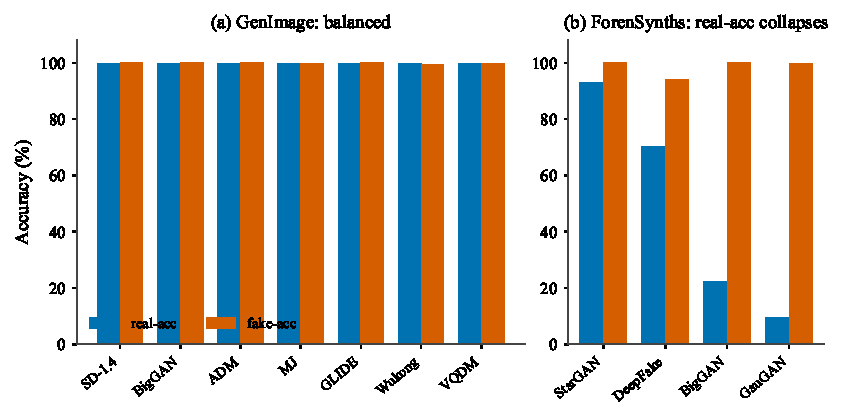
\includegraphics[width=\textwidth]{figs/fig_pergen.pdf}
  \caption{\textbf{Per-generator real- and fake-accuracy.} \textbf{(a)} On GenImage the
    detector is well balanced---real- and fake-accuracy are both $\approx$99--100\% on all
    seven generators. \textbf{(b)} On cross-architecture ForenSynths, fake-accuracy stays
    near 100\% while real-accuracy collapses (BigGAN 22.2\%, GauGAN 9.7\%): the model labels
    most images ``AI'', the signature of a detector leaning on a GenImage-specific cue that
    ForenSynths' real images do not share (\S{}4.2, \S{}4.3c).}
  \label{fig:pergen}
\end{figure}


\textbf{Double dissociation (numbers).} Comparing Route B and E-Delta on matched versus mismatched evaluation distributions (from the GATE-3 audit) yields a clean dissociation, reported here without interpretation (see \S{}4.3c): on a Q96-debiased validation set Route B scores \textbf{89.75\%} mean and E-Delta \textbf{99.78\%}; on the raw cross-generator OOD set Route B scores \textbf{99.73\%} and E-Delta \textbf{95.0\%} (\autoref{fig:dissoc}).

\subsection{Audit}

This section is the paper's core. We use the bottleneck's no-bypass guarantee (\S{}3.3) to measure, causally, what the detector's accuracy rests on.

\textbf{4.3a Channel reliance.} The learned classifier is \(\hat{y}=\sigma(\mathbf{w}^\top\mathbf{c}+b)\) with \(\mathbf{w}=[+6.45,+9.84,+6.21,+3.73,\mathbf{-13.53},+7.35]\) (order: bitplane-LSB, freq-radial, color-manifold, hf-noise, \textbf{jpeg-quant}, texture-geometry) and \(b=-5.06\) (seed-42 model; the other two seeds' rank-1 weights are reported below). The rank-1 weight belongs to jpeg-quant, but this is seed-dependent: in seed-1 the rank-1 weight belongs to freq-radial (+11.58), and in seed-2 freq-radial (+10.77) and texture-geometry ($-$10.51) nearly tie for the top two. In every seed, however, the top-two weights belong to the correlated compression pair \{jpeg-quant, freq-radial\}. Three interventions converge on a sharp picture.

\emph{Single-channel ablation.} In the seed-42 model, zeroing \texttt{jpeg-quant} collapses accuracy to chance on \textbf{every} generator (-49.2 to -49.8pp; 99.7\%\ensuremath{\rightarrow}50.2\% cumulative); zeroing \texttt{freq-radial} costs a substantial but smaller -4 to -30pp; the remaining four channels each cost about a point or less on most generators (texture-geometry the largest exception, up to -5.8pp on Wukong). Across three seeds, the compression pair \{jpeg-quant, freq-radial\} accounts for the dominant zero-out in every case (combined 66--88\,pp), while the other four channels remain below 3.3\,pp each (texture-geometry up to 7.8\,pp in one seed; \autoref{fig:reliance}). However, \textbf{which of the two correlated channels the head names as the carrier shifts}: seed-42 gives jpeg-quant $-$49.5\,pp and freq-radial $-$17.2\,pp; seed-1 reverses to freq-radial $-$38.7\,pp and jpeg-quant $-$24.5\,pp; seed-2 splits nearly evenly ($-$25.7 vs $-$24.7\,pp). The \emph{axis} of reliance is stable; the \emph{channel label} is not. So reliance is concentrated on a compression axis, not on a single named channel.

% Channel-reliance figure (data: 04_Stage4_Evidence.md multi-seed zero-out table).
\begin{figure}[t]
  \centering
  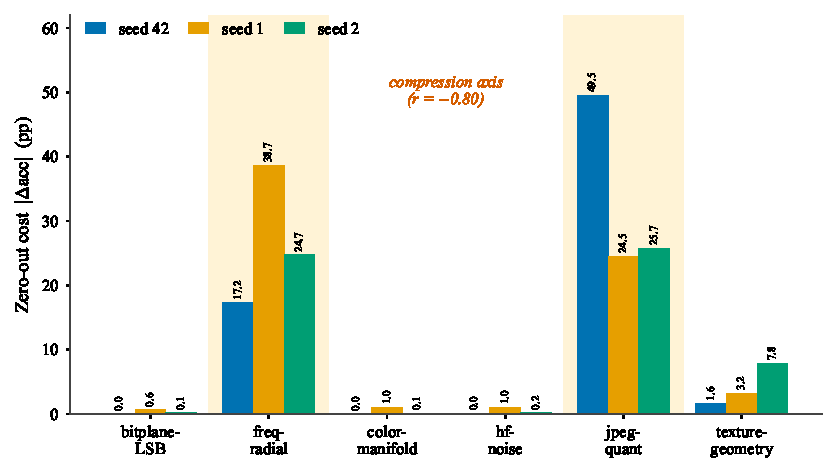
\includegraphics[width=\textwidth]{figs/fig_channel_reliance.pdf}
  \caption{\textbf{Causal channel reliance is concentrated on a compression axis, across
    three seeds.} Accuracy drop (pp) from zeroing each bottleneck channel, mean over the
    seven evaluation generators, for seeds 42/1/2. In every seed the two tall bars are the
    correlated compression pair \texttt{freq-radial} and \texttt{jpeg-quant} (shaded;
    $r{=}{-}0.80$), which dwarf the other four channels (all $|\Delta|<3.3$\,pp). Which
    member of the pair carries the larger drop \emph{shifts} across seeds (seed-42:
    \texttt{jpeg-quant}; seed-1: \texttt{freq-radial}; seed-2: nearly tied): the compression
    \emph{axis} is stable, the named \emph{carrier} is not. The linear-head weights do not
    reveal this ordering; only causal ablation does (\S{}4.3a).}
  \label{fig:reliance}
\end{figure}


\emph{Keep-only-one.} Restricting the classifier to one channel disentangles their roles: in the seed-42 model, \texttt{freq-radial} alone reaches \textbf{81.6--99.7\%} across generators---it is the continuous discriminator---whereas \texttt{jpeg-quant} alone yields exactly 50\% (its negative weight plus the bias labels everything ``real''). \texttt{jpeg-quant} thus acts as a \textbf{decision-flipper} that, in concert with \texttt{freq-radial}, sets the operating point, rather than as a standalone classifier. Standalone separability is itself seed-dependent (seed-2: bitplane-LSB alone $\approx$95\%; seed-1: no single channel above 53\%), reinforcing that weight magnitude and single-channel accuracy are unreliable proxies for functional role.

\emph{Counterfactual swap.} Replacing a single channel's value with the opposite class's mean confirms the causal lever (seed-42 model; the swap metric depends on class-conditional means that vary with the weight configuration): swapping \texttt{jpeg-quant} flips \textbf{23.9--72.5\%} of real predictions and 9.8--44.9\% of fake predictions, while every other channel---\texttt{freq-radial} included---flips under \ensuremath{\sim}2\% (at most 9\% on one generator).

Finally, \texttt{jpeg-quant} and \texttt{freq-radial} are \textbf{-0.80 correlated}: the two load-bearing channels encode the \emph{same} low-level cue---a compression/container signal---in scalar and spectral form, and the other four channels are essentially inert despite being trained by the concept-MSE loss. We stress that naming this cue \emph{compression} does not rest on the channels' supervision-induced labels---which \S{}5 argues should not be read literally---but on the independent perturbation evidence of \S{}4.3b: balanced accuracy collapses precisely when JPEG quality is lowered or high-frequency content is destroyed (\autoref{fig:confound}), the operations that specifically target compression artifacts. Two lessons follow. First, \textbf{weight magnitude is an unreliable proxy for functional role}: in the seed-42 model, \texttt{jpeg-quant} has the largest \(|w|\) yet cannot classify alone, while \texttt{freq-radial} carries the standalone signal; but which channel holds the largest \(|w|\) shifts across seeds, while the pair-level ablation pattern is stable---only intervention reveals this. Second, the detector is effectively a compression-axis classifier: the six ``concepts'' are not six independent pieces of evidence, but two correlated channels that encode a single cue in different representations.

\textbf{4.3b Confound battery.} If the load-bearing cue is a compression/container artifact, perturbing that artifact should degrade the detector. It does (Table 3). Re-encoding every image to a uniform JPEG quality of 95 (closing the PNG-vs-JPEG container gap) drops mean accuracy \textbf{-10.16pp} (worst on BigGAN -19.4 and ADM -14.0); re-saving as PNG with no other change costs \textbf{0.00pp} (a control); downsampling to 128\textsuperscript{2} (destroying high-frequency content) collapses accuracy \textbf{-44.64pp}, driven by a real-accuracy collapse---a probe of the detector's high-frequency reliance rather than of the container confound specifically; and using disjoint real-image pools across OOD generators changes results by \textbf{+0.12pp}, ruling out a shared-real-pool artifact (full JPEG-quality and resolution sweeps in \autoref{fig:confound}).

% Table 3 --- confound battery (B1/B2/B5). Numbers from B_confound_summary.md.
\begin{table}[t]
  \centering
  \caption{Confound battery: change in mean accuracy ($\Delta$acc, percentage points) under controlled
  perturbations of the image container and resolution. Closing the PNG-vs-JPEG container gap (JPEG-q95) and
  destroying high-frequency content (res128) both degrade the detector substantially, while a pure PNG re-save
  (control) and disjoint real-image pools do not.}
  \label{tab:confound}
  \small
  \begin{tabular}{lccc}
    \toprule
    Perturbation & mean $\Delta$acc & train-gen & OOD \\
    \midrule
    JPEG-q95 (close container gap)  & $-10.16$ & $-10.83$ & $-9.28$ \\
    PNG re-save (control)           & $+0.00$  & $+0.00$  & $+0.00$ \\
    res128 (destroy high-freq)      & $-44.64$ & $-43.91$ & $-45.62$ \\
    independent real pool           & ---      & ---      & $+0.12$ \\
    \bottomrule
  \end{tabular}
\end{table}


% Confound sweeps (data: batch1_analysis/B3_jpeg_quality_curve.csv, B4_resolution_curve.csv).
\begin{figure}[t]
  \centering
  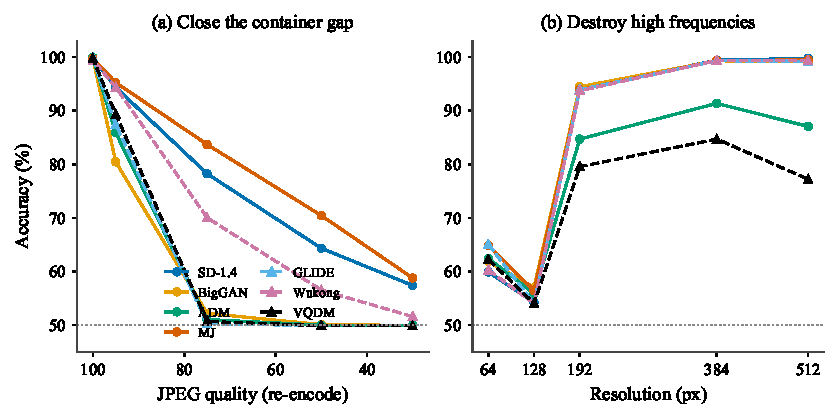
\includegraphics[width=\textwidth]{figs/fig_confound.pdf}
  \caption{\textbf{Confound battery as full sweeps: accuracy is carried by
    container/compression cues.} \textbf{(a)} Re-encoding every image to a decreasing JPEG
    quality (native $\sim$95+ on the left) drives accuracy toward chance, fastest on BigGAN,
    ADM, GLIDE, and VQDM; Stable Diffusion and Midjourney retain the most accuracy.
    \textbf{(b)} Down-sampling to destroy high-frequency content collapses accuracy at
    128\,px (a real-accuracy collapse) and recovers by 192\,px. Solid lines are
    training-family generators, dashed lines are unseen OOD generators; the single
    operating points in Table 3 are the 95-quality and 128-px slices of these curves
    (\S{}4.3b).}
  \label{fig:confound}
\end{figure}


\textbf{4.3c Persistence under debiasing, and the inflation/generalization split.} We then ask the question Grommelt's black-box analysis could not: does the reliance survive removing the confound at the data level? We retrain on the Q96-debiased corpus (E-Delta) and re-audit. The \texttt{jpeg-quant} weight shrinks---from -13.53 to -9.11 (a 1.49\ensuremath{\times} reduction)---which, taken alone, would suggest reduced reliance. \textbf{Intervention says otherwise:} on the debiased model, zeroing \texttt{jpeg-quant} still costs \textbf{-48.18pp} (it remains rank-1 by ablation), while \texttt{freq-radial}'s contribution falls to -0.90pp (it becomes inert once the container signal is debiased), and \texttt{jpeg-quant}'s per-generator real-vs-fake separation stays large (Cohen's \(d\) -3.84 to -5.47). We label this \textbf{Outcome C (persistence)}: the channel is \emph{not reducible} to the trivial PNG-vs-JPEG container label, since the model rebuilds its dependence on the same channel from a corpus in which that label has been neutralized. Whether the surviving signal reflects generative-pipeline traces, residual compression-history statistics that outlast uniform re-encoding, or a \emph{Q96 re-encoding signature} introduced by the debiasing step itself, is \textbf{unresolved}, and we do not claim the former. This also reads the double-dissociation of \S{}4.2: Route B (trained on the confounded corpus) wins on raw-OOD that shares the confound, E-Delta wins on Q96-matched data, and \textbf{both} route their decision through the compression axis---debiasing re-tunes the channel rather than removing reliance on it. \textbf{Outcome C replicates across seeds, with seed-dependent strength.} We retrained the debiased model on two further seeds (seed-1 for the full 10 epochs; seed-2 to epoch 6, where training was interrupted) and re-ran the identical audit. In \emph{every} seed a compression-pair channel is the rank-1 single-channel zero-out on the debiased model---\texttt{jpeg-quant} $-48.2$\,pp (seed-42), \texttt{freq-radial} $-14.2$\,pp (seed-1), \texttt{jpeg-quant} $-7.7$\,pp (seed-2; Appendix~\ref{app:edelta})---so data-level debiasing does \emph{not} eliminate compression-axis reliance. Its \emph{magnitude}, however, is seed-dependent, and seed-42 is the strong end: in seeds 1 and 2 the debiased model spreads the cue more evenly and the dominant single-channel cost falls to 8--14\,pp. The robust claim is thus qualitative---after debiasing the compression axis remains the top cue and is not reducible to the container label---rather than the specific $-48$\,pp, which is seed-42-specific; this mirrors the carrier seed-dependence we report for the raw model (\S{}4.3a). Detection stays competitive on all three debiased seeds (Q96-val mean 99.67--99.78\%).

% Route B vs E-Delta double dissociation (data: edelta/gate3_audit/gate3_full_audit.json).
\begin{figure}[t]
  \centering
  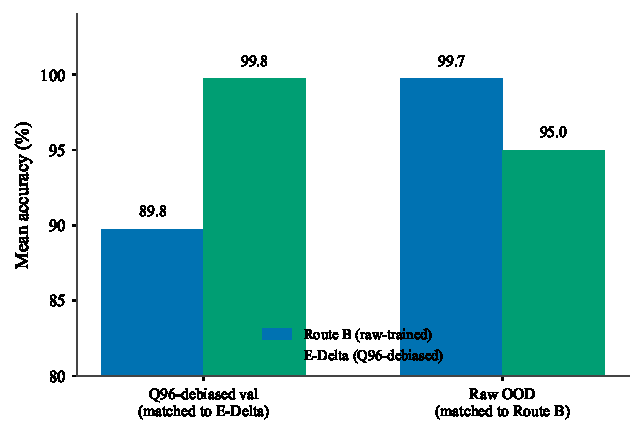
\includegraphics[width=0.62\textwidth]{figs/fig_dissociation.pdf}
  \caption{\textbf{Double dissociation between Route B and E-Delta.} On a Q96-debiased
    validation set (matched to E-Delta's training) the debiased model wins (99.8 vs 89.8);
    on the raw cross-generator OOD set (matched to Route B's training) Route B wins (99.7 vs
    95.0). Each model is strongest on the container statistics it was trained under, yet both
    route their decision through the same compression channel---debiasing \emph{re-tunes} the
    channel rather than removing reliance on it (\S{}4.3c).}
  \label{fig:dissoc}
\end{figure}


The cross-architecture result bounds how much of the headline number is confound-inflated. Route B's accuracy falls from \textbf{99.67\%} on GenImage-OOD to \textbf{73.65\%} on ForenSynths---a 26-point drop on a container-mismatched benchmark, consistent with the confound battery. We are careful not to attribute the entire gap to the confound: ForenSynths is also a genuine GAN-versus-diffusion distribution shift, so the clean confound isolation remains B1/B2 and \S{}4.3a, with ForenSynths as corroborating external evidence. The honest reading is \textbf{partial confound inflation alongside genuine partial generalization} (\autoref{fig:generalization}; quantified next).

% Cross-benchmark generalization figure (data: body.tex 4.2/4.3c/4.4).
\begin{figure}[t]
  \centering
  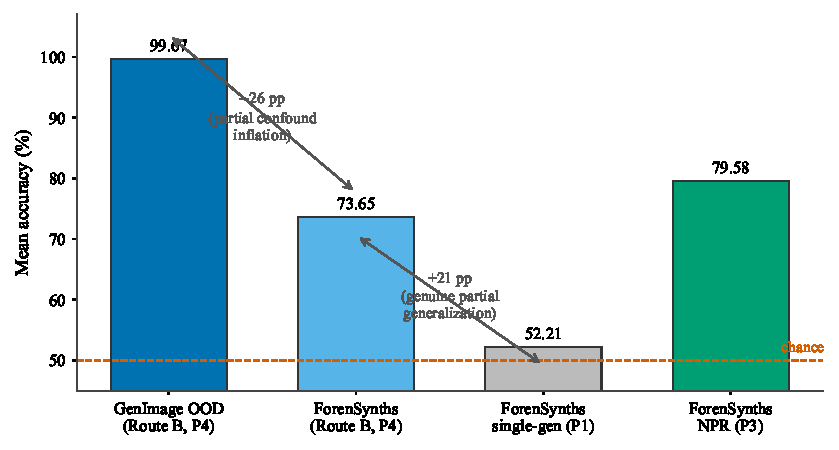
\includegraphics[width=0.93\textwidth]{figs/fig_generalization.pdf}
  \caption{\textbf{Partial confound inflation alongside genuine partial generalization.}
    Route B reaches 99.67\% mean on held-out GenImage generators but only 73.65\% on
    cross-architecture ForenSynths---a 26-point drop on a container-mismatched benchmark,
    consistent with the compression confound. Yet 73.65\% is far above an otherwise-identical
    single-generator model (52.21\%, near chance), so multi-generator training buys
    \emph{genuine} partial cross-architecture transfer ($+21$\,pp). NPR, trained on ProGAN and
    thus domain-matched to ForenSynths' GANs, scores 79.58\%---above Route B---so the transfer
    is partial, not best-in-class (\S{}4.3c, \S{}4.4).}
  \label{fig:generalization}
\end{figure}


\subsection{Ablations (what the data support)}

\textbf{Generator coverage (single- vs.~multi-generator), on a common benchmark.} Evaluated identically on ForenSynths, an otherwise-comparable single-generator (SD-1.4-only) model reaches only \textbf{52.21\% (AUC 0.528)}---essentially chance, classifying almost every GAN image as real---whereas the four-generator Route B reaches \textbf{73.65\% (AUC 0.820)} (Table 4). Multi-generator training therefore buys \emph{genuine} partial cross-architecture generalization (+21.4pp). For reference, NPR \citep{tan2024npr}, trained on ProGAN and thus domain-matched to ForenSynths' GANs, scores \textbf{79.58\% (AUC 0.894)} on the same benchmark---above Route B, underscoring that Route B's generalization is partial rather than complete. We flag that the single-vs-multi contrast is suggestive rather than perfectly controlled: the two models also differ in training code, loss, and data scale, so we read it as directional evidence, not a clean one-factor ablation.

% Table 4 --- single- vs multi-generator on a common cross-architecture benchmark (ForenSynths).
% Numbers: cbnet_forensynths.json (52.21), cbnet_multigen_forensynths.json (73.65), npr_forensynths.json (79.58).
\begin{table}[t]
  \centering
  \caption{Single- versus multi-generator training, evaluated identically on ForenSynths (cross-architecture).
  Multi-generator training (P4) buys genuine partial cross-architecture generalization over a single-generator
  model (P1); NPR (P3, ProGAN-trained and thus domain-matched to ForenSynths' GANs) is stronger still,
  underscoring that our generalization is partial, not best-in-class. The contrast is directional, not a clean
  one-factor ablation (the models differ in training code, loss, and data scale as well as generator coverage).}
  \label{tab:forensynths}
  \small
  \begin{tabular}{lccc}
    \toprule
    Model (ForenSynths) & Train protocol & Mean Acc (\%) & Mean AUC \\
    \midrule
    CBNet single-gen (SD-1.4) & P1 & 52.21 & 0.528 \\
    CBNet Route B (4 gens)    & P4 & 73.65 & 0.820 \\
    NPR (ProGAN)              & P3 & 79.58 & 0.894 \\
    \bottomrule
  \end{tabular}
\end{table}


\textbf{Ablations not run.} Our concept set (\(K{=}6\)), the dual-stream backbone, and the loss components were fixed \emph{a priori}; we did not run controlled ablations over \(K\), backbone variants, or the individual loss terms (\(L_{\text{pair}}\), \(L_{\text{sparsity}}\)). We \emph{did} ablate the bottleneck itself (\S{}4.5), finding it accuracy-neutral; but we make no empirical claim about the optimality of \(K{=}6\) or the contribution of the auxiliary losses, and discuss these as limitations (\S{}6) and future work rather than asserting unsupported results.

\subsection{What the bottleneck adds}

The no-bottleneck baseline (\S{}4.1) achieves comparable detection accuracy: 99.60\% OOD mean versus CBNet's 99.67--99.82\% across three seeds, confirming that the concept bottleneck is accuracy-neutral. Under the JPEG-q95 confound battery (\S{}4.3b), the baseline shows \emph{equal or greater} accuracy loss: mean accuracy drops to 87.25\% versus CBNet's 88.99\% (Table~3), with fake-accuracy falling from 78.4\% to 74.8\% averaged across generators. The bottleneck is therefore not the source of the compression shortcut; the backbone and/or training data are.

The bottleneck's contribution is \emph{interpretive}, not \emph{predictive}: it provides a structured 6-dimensional concept vector that enables the closed-form audit protocol of \S{}3.7---zero-out, counterfactual swap, weight reading---at no accuracy cost and no additional confound vulnerability. Without it, the same backbone exploits the same shortcut, but auditing requires opaque gradient-based attribution that lacks the bottleneck's no-bypass guarantee.

\textbf{Does post-hoc attribution recover the same account?} This admits a direct test. From the no-bottleneck baseline's 2560-dimensional pooled features we fit linear probes to the six dataset-level concept heuristics (\S{}3.4) on a held-out split (Appendix~\ref{app:probe}). The forensic statistics are substantially decodable---held-out probe $R^2$ of \textbf{0.88} for \texttt{jpeg-quant} and 0.61 for \texttt{freq-radial} (0.35--0.81 for the others)---so the evidence the bottleneck names is already \emph{latent} in the plain backbone, consistent with the baseline's equal confound-susceptibility above. What the plain backbone does not furnish is a \emph{causal locus}: the decoded compression direction is nearly orthogonal to the baseline's decision direction ($|\cos|\,{\approx}\,0.003$, against ${\approx}\,0.02$ for a random direction), and because the baseline saturates on held-out GenImage ($\approx$99.9\% balanced accuracy), projecting that direction out---or, as a control, any random direction---leaves the decision unchanged. The no-skip bottleneck scalar is, by construction, the causal locus the baseline lacks: zeroing it removes 49.5\,pp. We therefore read the audit's value precisely as \emph{interpretive}, not predictive: the bottleneck does not expose a cue the backbone cannot use, it supplies a built-in, named, causally-ablatable handle on a cue the backbone already uses---and post-hoc attribution, which here recovers the cue's \emph{presence} but no single ablatable locus, is a weaker instrument on this architecture.

\section{Discussion}

Our results admit one honest summary: the detector exhibits \textbf{partial confound inflation alongside genuine partial generalization.} Neither extreme holds. It is not a pure container detector---multi-generator training yields real cross-architecture transfer (\S{}4.4)---nor is it a robustly general one---much of its headline GenImage number does not survive a change of benchmark (\S{}4.3c). The contribution of this paper is the ability to say \emph{which} part is which, and to do so from inside a single competitive model.

\textbf{Intervention is the authority, not weights.} The clearest methodological lesson is that the linear head's weights describe only its parameters, not the model's functional reliance, and that the appropriate test is causal---single-channel ablation and counterfactual swaps. The point is not abstract: reading the weights would have mis-described the model in two opposite directions. The channel with the largest weight magnitude shifts across seeds (seed-42: \texttt{jpeg\_quant}; seed-1: \texttt{freq\_radial}; seed-2: \texttt{freq\_radial}), yet in every seed the top-two zero-out channels are the same correlated compression pair---weight magnitude alone would have pointed to a different ``dominant'' channel in each seed, while only intervention reveals the pair-level reliance, which is stable across the three seeds we tested. And after Q96 debiasing the \texttt{jpeg\_quant} weight shrinks by 1.49\ensuremath{\times}, which alone would suggest the model had weaned off it, whereas ablation shows its functional contribution essentially unchanged. A post-hoc attribution that inspects weights (or, by extension, a narration that is never intervened upon) would have reported both of these backwards. Only intervention recovers the functional structure.

\textbf{A compression-axis, single-cue decision.} That structure is narrow. The decision is carried by a compression axis---the correlated pair \texttt{jpeg\_quant} and \texttt{freq\_radial} ($r = -0.80$)---and which of the two the linear head names as the primary carrier shifts across random seeds; the remaining four channels are near-inert despite being trained. The model, in other words, discovered that one cue suffices and concentrated its decision into a correlated pair rather than using six independent pieces of evidence. This is the empirical reason ``interpretable by construction'' is the wrong claim for a concept bottleneck: the architecture constrains the decision to pass through named channels, but \emph{what} those channels encode and \emph{how many} matter are outcomes of training that have to be measured, not read off the design. Functional reliance on a compression signal does not imply semantic faithfulness to ``JPEG-quantization traces'' as a human-interpretable concept---the same functional role can be served by either of two correlated channels, and the model is indifferent to which one the auditor names. The \texttt{freq\_radial} channel---a radial power-spectrum slope---also ties this result to the spectral-artifact line of AGID \citep{frank2020dctgan, durall2020watch}, which attributes detectability to up-sampling fingerprints in the frequency domain: our audit is consistent with that mechanism, but adds the cautionary qualifier that on GenImage the spectral signal is substantially entangled with JPEG compression (\S{}4.3b) rather than being a clean generative trace.

\textbf{What persistence under debiasing does and does not show.} Retraining on the Q96-debiased corpus removes the trivial explanation. If \texttt{jpeg\_quant} were merely the PNG-versus-JPEG container label, neutralizing that label at the data level should dissolve the model's reliance on it; instead the model rebuilds its dependence on the same compression axis: across three seeds a compression-pair channel remains the rank-1 single-channel zero-out on the debiased model, though the magnitude is seed-dependent (8--48\,pp; Outcome C, \S{}4.3c). We therefore conclude that the dominant cue is a frequency/compression-domain signal \textbf{not reducible} to container format. We deliberately stop there. Uniform re-encoding standardizes the final compression step but not the images' cumulative processing history, so the surviving signal could be genuine generative-pipeline traces, residual compression-history statistics that outlast re-encoding, or a mixture; our experiments do not separate these, and we do \textbf{not} claim the channel captures generative semantics. The honest claim is bounded---deeper than the container label, shallower than a proof of generative-trace detection.

\textbf{External validity: what ForenSynths adds.} Moving to a benchmark whose images do not share GenImage's acquisition statistics, the detector falls from 99.67\% to 73.65\%. We read this as corroboration that the GenImage-OOD headline is partly inflated by the shared confound---but only corroboration, because ForenSynths is also a genuine GAN-versus-diffusion distribution shift; the clean confound isolation remains the within-GenImage perturbations (\S{}4.3a--b). At the same time, 73.65\% is far above the 52.21\% of a single-generator model, so multi-generator training does buy genuine partial cross-architecture generalization. We present one comparison plainly: NPR, a ProGAN-trained detector domain-matched to ForenSynths' GANs, scores 79.58\% on the same benchmark---above our model. Our generalization is therefore partial and not best-in-class on this cross-architecture set, and we make no claim to the contrary. None of these results is a weakness of the audit; each is something the audit was built to reveal.

\textbf{Design intent is not a substitute for measurement.} The architecture included two terms intended to discourage shortcut reliance---a cross-generator content-pairing consistency loss and an activation-entropy regularizer---yet the trained model still concentrated onto a single confound-aligned channel. We did not run ablations isolating these terms and so make \textbf{no} quantitative claim that they succeeded or failed (\S{}6). But the qualitative observation matters: stated inductive biases toward diverse, generator-invariant evidence did not prevent the collapse. There are intelligible reasons---an entropy term rewards diverse \emph{activations}, which is silent about whether the \emph{decision} is diverse, and a consistency term that rewards generator-invariance is trivially satisfied by a generator-invariant confound. The general lesson is the one this paper is built on: an architecture's design intent is a hypothesis about its behavior, and behavior must be audited rather than assumed.

\textbf{Relation to Grommelt.} \citet{grommelt2024fakejpeg} established that GenImage and similar datasets conflate generated-ness with JPEG/format and size artifacts, and that black-box detectors learn them---a diagnosis at the level of the dataset. Our contribution is the model-internal counterpart: we localize that confound to a specific evidence channel, quantify its causal contribution by intervention, and show through the Q96 retrain that the reliance persists rather than dissolving once the dataset is debiased. The two views are complementary, and ours answers questions---\emph{where} in the model, \emph{how much}, and \emph{does it survive debiasing}---that a black-box analysis structurally cannot. We frame the contribution narrowly and accordingly: it is a method for model-internal confound localization, and what that method reveals about \emph{one} competitive detector on GenImage---not a multi-detector or multi-dataset survey. That broader study is what this single-detector audit is meant to motivate, not to deliver.

\textbf{The bottleneck as a testability surface.} Taken together, these findings reposition the concept bottleneck for AGID. Its value here is not that it renders the detector interpretable---our audit shows it does not, in the naive sense of six meaningful concepts---but that it furnishes a \emph{testability surface}: a small set of channels through which the decision must pass and on which faithfulness can be causally probed. On GenImage, that surface let us turn ``the benchmark may be confounded'' from a suspicion into a measurement, and to separate, inside one competitive detector, the portion of its competence that is artifact from the portion that genuinely generalizes.

\textbf{What the bottleneck does not cost.} A no-bottleneck baseline achieves comparable OOD accuracy (99.60\% versus 99.67--99.82\%) and is equally susceptible to the compression confound (Table~3), confirming that the bottleneck's contribution is interpretive rather than predictive. The concept bottleneck enables the audit protocol at zero accuracy cost.

\textbf{Implications for practice.} Two uses follow for the people who build and consume these benchmarks. For \emph{benchmark builders}, a per-channel causal audit turns ``this dataset may be confounded'' from a suspicion into a localized, quantified target: one can report how much of a reference detector's accuracy a candidate benchmark routes through a removable acquisition cue, and iterate on dataset construction until that share falls. For \emph{detector developers}, the interventionable bottleneck is a cheap pre-deployment stress test---ablate each evidence channel and re-measure---that flags reliance on a single removable cue \emph{before} a model meets a distribution that lacks it, precisely the failure our ForenSynths transfer exposes. Neither use requires the channels to be individually faithful; both require only that the decision be forced through a small, separately-ablatable set.

\section{Limitations}

We frame our contribution as an audit, and an audit's credibility rests on stating plainly what it does not establish. We list the limitations from most to least consequential for our claims.

\textbf{Protocol comparability.} Our detector trains on four generators (protocol P4), whereas the baselines we tabulate train on one (P1) or per-generator (P2). Consequently CBNet's held-out set (GLIDE/Wukong/VQDM/SD-1.5) is narrower than the cross-generator set those baselines are evaluated on, and the comparison in Table 1 is not head-to-head; this is precisely why we claim \emph{competitive}, not state-of-the-art, detection. The single- versus multi-generator contrast of \S{}4.4 is likewise not a clean one-factor ablation---the two models differ in training code, loss, and data scale as well as in generator coverage---so we read its +21-point gap as directional evidence of partial generalization rather than a controlled measurement.

\textbf{Untested architectural and loss choices.} Several design decisions were fixed \emph{a priori} and never ablated: the number of channels (\(K{=}6\)), the dual-stream backbone, the presence of the bottleneck itself (versus a same-backbone classifier with post-hoc attribution), and the two auxiliary loss terms. We therefore make no empirical claim that \(K{=}6\) is optimal, that the bottleneck is necessary for accuracy, or that the content-pairing and entropy regularizers help or hurt the result. In particular, because we ran no ablation isolating \(L_{\text{pair}}\) or \(L_{\text{sparsity}}\), our observation that the model collapsed onto a single cue \emph{despite} these terms is qualitative: it motivates auditing but does not quantify the regularizers' effect.

\textbf{Confound and distribution shift are entangled on ForenSynths.} The 26-point GenImage-to-ForenSynths drop is consistent with confound inflation, but ForenSynths also differs from GenImage in generator architecture (GAN-heavy) and image source, so the drop conflates confound removal with a genuine distribution shift. We do not attribute the full gap to the confound; the clean confound isolation rests on the within-GenImage perturbations (\S{}4.3b) and the intervention analysis (\S{}4.3a), with ForenSynths serving only as corroborating external evidence.

\textbf{Attribution ceiling of Q96 debiasing.} Our persistence result (Outcome C) shows the dominant channel is not reducible to the final PNG-versus-JPEG container label; but uniform Q96 re-encoding standardizes only the final compression step and does not erase the images' cumulative processing history. We therefore cannot determine whether the surviving signal reflects generative-pipeline traces or residual compression-history statistics, and we make no claim that it is the former. Disentangling them would require generators and real images with matched, fully controlled processing pipelines, which is beyond this work.

\textbf{Concept identity is supervision-induced.} The six channels acquire their meaning from weak heuristic supervision rather than from the architecture, and our own audit shows that meaning is not preserved under the task objective---two channels dominate and four are inert. We therefore do not claim six individually faithful, human-meaningful concepts. The audit \emph{characterizes} this gap; it does not repair it, and producing concepts that are simultaneously faithful and individually informative for AI-generated image detection remains open.

\textbf{Dataset and real-image scope.} Training and most evaluation draw on GenImage, with real images from ImageNet, so the specific confound we localize is a property of how GenImage was assembled. \citet{grommelt2024fakejpeg} report similar biases in comparable datasets, which suggests the phenomenon is not unique to GenImage; but we have not verified our model-internal account on other corpora and make no claim beyond GenImage and the ForenSynths transfer test. Relatedly, the four generators span an 8\ensuremath{\times} range of native resolution, and GenImage's real and synthetic images differ systematically in container format---dataset-level properties we cannot remove inside the model, and which degrade the high-frequency channels unevenly across generators.

\textbf{Scale of the audit evidence.} An early smoke-scale experiment suggested the model's reliance ``migrated'' to other channels after debiasing; this did not survive at full scale, and we attribute it to evaluation on the training set. Only the full-scale audit reported here stands. We flag this explicitly to discourage over-reading small-scale concept-reliance signals.

\textbf{Label--crop misalignment.} Concept labels were precomputed on a center crop while training applied a random crop, so the supervision targets approximate, rather than exactly match, the pixels the model saw at each step. We expect this to add mild label noise but not to change the qualitative findings.

\section{Conclusion}

AI-generated image detection on GenImage is, by the leaderboard, nearly solved. We asked a different question: not how high the accuracy is, but what it is made of. To answer it we built a deliberately conventional, single-GPU detector and equipped it with a concept bottleneck whose one essential property is a no-skip guarantee---every prediction passes through six separately-testable evidence channels and nothing else. The detector is competitive, but it is the \emph{subject} of our study, not its contribution; the contribution is the architecture-level audit surface, and the causal intervention evidence it makes possible.

Using that surface, we localized a competitive detector's decision to a compression-axis channel pair (jpeg-quant and freq-radial, $r{=}{-}0.80$), quantified its reliance by ablation and counterfactual rather than by weight inspection, and showed that the reliance persists even after Grommelt-style debiasing neutralizes the obvious container cue (Outcome C, replicated across three seeds with seed-dependent strength). Across three random seeds, the pair-level compression-axis reliance is stable, but which of the two correlated channels the head names as the carrier shifts---an empirical demonstration that weight inspection alone is unreliable. The honest summary is partial confound inflation alongside genuine partial generalization: a substantial part of the headline GenImage performance does not transfer to a container-mismatched benchmark, yet multi-generator training does buy real---if incomplete---cross-architecture generalization. The methodological lesson outlasts this particular model: weight magnitudes and post-hoc narrations \emph{describe} a model, whereas only intervention \emph{tests} it, and an interventionable bottleneck is what turns an explanatory claim into a checkable object.

Our work extends, rather than discovers, the GenImage confound. \citet{grommelt2024fakejpeg} established it at the dataset level with black-box detectors; we provide the model-internal counterpart---where the reliance lives, how large it is, and whether it survives debiasing---which a black-box analysis structurally cannot. Several directions follow: controlled ablations over the loss terms, backbone, channel count, and the bottleneck itself; experiments that disentangle generative-pipeline traces from residual compression history; and applying the same audit to other detectors and datasets, so as to ask of the field's near-saturated numbers, in general, what they are made of.


\medskip

\bibliographystyle{plainnat}
\bibliography{ref}

% =====================================================================
%  APPENDIX -- supplementary tables. Every number is transcribed from a
%  verified disk artifact under AGID_Project/Code/Results/ (cited per table).
%  No main-text claim depends on this material; it only adds detail.
% =====================================================================
\appendix

\section{Training and Hyperparameter Configuration}
\label{app:hyper}

Table~\ref{tab:hyper} records the as-run configuration for both models
(\S{}3.5--3.6). The two instances differ only in training data and epoch budget.

\begin{table}[h]
  \centering
  \caption{As-run training configuration. Source: training scripts / \S{}3.5--3.6.}
  \label{tab:hyper}
  \small
  \begin{tabular}{ll}
    \toprule
    Component / setting & Value \\
    \midrule
    Pixel stream            & ResNet-50, ImageNet-pretrained ($\to 2048{\times}8{\times}8$) \\
    Signal stream           & NPR residual $\to$ 5-layer strided CNN ($\to 512{\times}8{\times}8$) \\
    Bottleneck              & $K{=}6$ heads: $1{\times}1$ conv($2560{\to}640$), BN, ReLU, $1{\times}1$ conv, GAP, $\sigma$ \\
    Parameters              & 38.0M (CBNet-AGID) / 28.2M (BaselinePlain, no bottleneck) \\
    Optimizer               & AdamW, weight decay $10^{-4}$, cosine schedule \\
    Learning rates          & $10^{-4}$ backbone / $5\times10^{-4}$ bottleneck / $10^{-3}$ classifier \\
    Precision / batch       & bfloat16 AMP; batch 32 $\times$ grad-accum 2 (effective 64) \\
    Input size              & $256\times256$ \\
    Augmentation            & random crop, horizontal flip, ImageNet norm \\
                            & (JPEG-recompression and Gaussian-blur \emph{disabled}) \\
    Loss                    & $L_{\text{task}}+0.5\,L_{\text{concept}}+0.2\,L_{\text{pair}}+0.05\,L_{\text{sparsity}}$ \\
    Seeds                   & 42 (primary); 1, 2 (replications) \\
    Epochs                  & 20 (Route B) / 10 (E-Delta, Q96-debiased) \\
    Training data           & 4 GenImage generators (SD-1.4, BigGAN, ADM, MJ), 25k/class \\
    Hardware                & single RTX 4060 Laptop, 8\,GB VRAM \\
    \bottomrule
  \end{tabular}
\end{table}

\section{Per-Seed Classifier Weights and Concept Reliance}
\label{app:seeds}

Tables~\ref{tab:seed-weights} and~\ref{tab:seed-zeroout} give the full multi-seed audit
behind \S{}4.3a. The linear-head weights and the single-channel zero-out costs are both
seed-unstable in \emph{which} channel ranks first, while the compression pair
\{\texttt{freq-radial}, \texttt{jpeg-quant}\} is the top-two zero-out in every seed.
With only three seeds we do not report confidence intervals; the cross-seed spread in
Tables~\ref{tab:seed-weights}--\ref{tab:seed-zeroout} should be read as an illustrative
range, not a calibrated variance estimate.

\begin{table}[h]
  \centering
  \caption{Learned linear-head weights $\mathbf{w}$ and bias $b$ per seed (order:
    bitplane-LSB, freq-radial, color-manifold, hf-noise, jpeg-quant, texture-geometry).
    Source: \texttt{batch1\_analysis/A2\_classifier\_weights.json} (seed 42); multi-seed
    record in \texttt{04\_Stage4\_Evidence.md}.}
  \label{tab:seed-weights}
  \small
  \begin{tabular}{lrrrrrrr}
    \toprule
    Seed & bitplane & freq-rad. & color & hf-noise & jpeg-q. & texture & bias \\
    \midrule
    42 & $+6.45$ & $+9.84$ & $+6.21$ & $+3.73$ & $\mathbf{-13.53}$ & $+7.35$ & $-5.06$ \\
    1  & $+9.07$ & $\mathbf{+11.58}$ & $-6.89$ & $+7.29$ & $-9.63$ & $-9.36$ & $+1.07$ \\
    2  & $+9.43$ & $\mathbf{+10.77}$ & $+6.56$ & $+5.60$ & $-9.94$ & $-10.51$ & $-1.97$ \\
    \bottomrule
  \end{tabular}
\end{table}

\begin{table}[h]
  \centering
  \caption{Single-channel zero-out cost $\Delta$acc (pp), mean over the seven evaluation
    generators, per seed. The compression pair is bold. Source:
    \texttt{seed\{42,1,2\}\_analysis/A3\_concept\_zeroout.csv}.}
  \label{tab:seed-zeroout}
  \small
  \begin{tabular}{lrrrrrr}
    \toprule
    Seed & bitplane & freq-rad. & color & hf-noise & jpeg-q. & texture \\
    \midrule
    42 & $-0.01$ & $\mathbf{-17.24}$ & $-0.03$ & $-0.04$ & $\mathbf{-49.54}$ & $-1.58$ \\
    1  & $-0.64$ & $\mathbf{-38.66}$ & $-0.97$ & $-1.04$ & $\mathbf{-24.49}$ & $-3.23$ \\
    2  & $-0.14$ & $\mathbf{-24.73}$ & $-0.12$ & $-0.19$ & $\mathbf{-25.73}$ & $-7.81$ \\
    \bottomrule
  \end{tabular}
\end{table}

\section{Full Single-Channel Ablation (Seed 42)}
\label{app:ablation}

Table~\ref{tab:full-ablation} expands the seed-42 zero-out to every generator. Zeroing
\texttt{jpeg-quant} costs $\approx$49\,pp uniformly (it flips the operating point on all
generators); \texttt{freq-radial} costs a larger but generator-dependent amount; the other
four channels are inert ($|\Delta|<6$\,pp, mostly $<1$\,pp).

\begin{table}[h]
  \centering
  \caption{Per-generator single-channel zero-out $\Delta$acc (pp), seed-42 model. Source:
    \texttt{seed42\_analysis/A3\_concept\_zeroout.csv}.}
  \label{tab:full-ablation}
  \small
  \begin{tabular}{lrrrrrr}
    \toprule
    Generator & bitplane & freq-rad. & color & hf-noise & jpeg-q. & texture \\
    \midrule
    SD-1.4     & $0.00$  & $-24.60$ & $+0.05$ & $-0.05$ & $-49.60$ & $-2.60$ \\
    BigGAN     & $+0.15$ & $-30.25$ & $+0.15$ & $+0.10$ & $-49.70$ & $+0.15$ \\
    ADM        & $+0.05$ & $-21.50$ & $+0.05$ & $+0.05$ & $-49.80$ & $-0.90$ \\
    Midjourney & $-0.05$ & $-15.40$ & $-0.15$ & $0.00$  & $-49.45$ & $-0.80$ \\
    GLIDE      & $+0.10$ & $-4.20$  & $+0.15$ & $+0.05$ & $-49.55$ & $+0.15$ \\
    Wukong     & $-0.35$ & $-19.70$ & $-0.35$ & $-0.45$ & $-49.20$ & $-5.75$ \\
    VQDM       & $+0.05$ & $-5.05$  & $-0.10$ & $+0.05$ & $-49.50$ & $-1.30$ \\
    \midrule
    mean       & $-0.01$ & $-17.24$ & $-0.03$ & $-0.04$ & $-49.54$ & $-1.58$ \\
    \bottomrule
  \end{tabular}
\end{table}

\section{Concept Correlation Matrix}
\label{app:corr}

Table~\ref{tab:corr} is the Pearson correlation among the six channel activations on the
training data. The load-bearing pair \texttt{freq-radial}/\texttt{jpeg-quant} is the
strongest off-diagonal entry ($-0.80$), confirming the two encode one cue.

\begin{table}[h]
  \centering
  \caption{Pearson correlation of channel activations. Source:
    \texttt{batch1\_analysis/A5\_pearson.csv}.}
  \label{tab:corr}
  \small
  \begin{tabular}{lrrrrrr}
    \toprule
     & bitplane & freq-rad. & color & hf-noise & jpeg-q. & texture \\
    \midrule
    bitplane  & $1.00$  & $0.42$  & $0.59$  & $-0.17$ & $-0.57$ & $-0.11$ \\
    freq-rad. & $0.42$  & $1.00$  & $0.45$  & $-0.23$ & $\mathbf{-0.80}$ & $0.24$ \\
    color     & $0.59$  & $0.45$  & $1.00$  & $-0.23$ & $-0.60$ & $-0.10$ \\
    hf-noise  & $-0.17$ & $-0.23$ & $-0.23$ & $1.00$  & $0.41$  & $0.49$ \\
    jpeg-q.   & $-0.57$ & $\mathbf{-0.80}$ & $-0.60$ & $0.41$  & $1.00$  & $0.03$ \\
    texture   & $-0.11$ & $0.24$  & $-0.10$ & $0.49$  & $0.03$  & $1.00$ \\
    \bottomrule
  \end{tabular}
\end{table}

\section{Extended Detection, OOD, and Calibration}
\label{app:ext}

Table~\ref{tab:calib} gives per-generator calibration (the pooled ECE 0.0034 quoted in
\S{}4.1 is the last row). Table~\ref{tab:forensynths-full} gives the full ForenSynths
metrics behind \S{}4.2, and Table~\ref{tab:baseline-ood} the no-bottleneck baseline OOD
detail behind \S{}4.5.

\begin{table}[h]
  \centering
  \caption{Per-generator calibration (2000 images/generator). Source:
    \texttt{batch1\_analysis/C5\_calibration.json}.}
  \label{tab:calib}
  \small
  \begin{tabular}{lrrr}
    \toprule
    Generator & Brier & NLL & ECE \\
    \midrule
    SD-1.4     & $0.00124$ & $0.00651$ & $0.00472$ \\
    BigGAN     & $0.00111$ & $0.00538$ & $0.00256$ \\
    ADM        & $0.00092$ & $0.00573$ & $0.00292$ \\
    Midjourney & $0.00241$ & $0.01219$ & $0.00223$ \\
    GLIDE      & $0.00144$ & $0.00542$ & $0.00339$ \\
    VQDM       & $0.00188$ & $0.00753$ & $0.00428$ \\
    Wukong     & $0.00424$ & $0.01695$ & $0.00653$ \\
    \midrule
    pooled (14k) & $0.00189$ & $0.00853$ & $\mathbf{0.00335}$ \\
    \bottomrule
  \end{tabular}
\end{table}

\begin{table}[h]
  \centering
  \caption{ForenSynths per-generator metrics, Route B. Source:
    \texttt{cbnet\_multigen\_forensynths.json}.}
  \label{tab:forensynths-full}
  \small
  \begin{tabular}{lrrrrr}
    \toprule
    Generator & Acc & AUC & AP & real-acc & fake-acc \\
    \midrule
    StarGAN  & $96.42$ & $0.999$ & $0.997$ & $92.85$ & $100.0$ \\
    DeepFake & $82.24$ & $0.934$ & $0.946$ & $70.30$ & $94.22$ \\
    BigGAN   & $61.10$ & $0.692$ & $0.641$ & $22.20$ & $100.0$ \\
    GauGAN   & $54.82$ & $0.657$ & $0.582$ & $9.72$  & $99.92$ \\
    \midrule
    mean     & $73.65$ & $0.820$ & $0.791$ & $48.77$ & $98.53$ \\
    \bottomrule
  \end{tabular}
\end{table}

\begin{table}[h]
  \centering
  \caption{No-bottleneck baseline (BaselinePlain) on GenImage OOD generators. Source:
    \texttt{ood\_eval\_baseline\_nobottleneck.json}.}
  \label{tab:baseline-ood}
  \small
  \begin{tabular}{lrrrr}
    \toprule
    Generator & Acc & AUC & real-acc & fake-acc \\
    \midrule
    GLIDE  & $99.90$ & $1.000$ & $99.80$ & $100.0$ \\
    Wukong & $99.00$ & $1.000$ & $99.80$ & $98.20$ \\
    VQDM   & $99.90$ & $1.000$ & $99.80$ & $100.0$ \\
    \midrule
    mean   & $99.60$ & $1.000$ & $99.80$ & $99.40$ \\
    \bottomrule
  \end{tabular}
\end{table}

\section{E-Delta (Q96-Debiased) Full Audit}
\label{app:edelta}

Tables~\ref{tab:edelta-weights}--\ref{tab:dissoc} expand Outcome C (\S{}4.3c). After
debiasing, the \texttt{jpeg-quant} weight shrinks $1.49\times$ yet its zero-out cost stays
$-48.18$\,pp (rank-1 by ablation), while \texttt{freq-radial} becomes inert; the Cohen's
$d$ for \texttt{jpeg-quant} remains large and negative on every generator. The
double-dissociation detail (Table~\ref{tab:dissoc}) shows each model winning on the
container statistics it was trained under.

\begin{table}[h]
  \centering
  \caption{Linear-head weights, Route B vs E-Delta (Q96-debiased), and the debiased
    single-channel zero-out cost. Source:
    \texttt{edelta/gate3\_audit/gate3\_full\_audit.json}.}
  \label{tab:edelta-weights}
  \small
  \begin{tabular}{lrrr}
    \toprule
    Channel & $w$ (Route B) & $w$ (E-Delta) & $\Delta$acc zero-out (E-Delta, pp) \\
    \midrule
    bitplane-LSB     & $+6.45$  & $+4.98$ & $-0.23$ \\
    freq-radial      & $+9.84$  & $+6.37$ & $-0.90$ \\
    color-manifold   & $+6.21$  & $+5.07$ & $-0.28$ \\
    hf-noise         & $+3.73$  & $+2.83$ & $-0.25$ \\
    jpeg-quant       & $-13.53$ & $-9.11$ & $\mathbf{-48.18}$ \\
    texture-geometry & $+7.35$  & $+5.32$ & $-0.35$ \\
    \midrule
    bias             & $-5.06$  & $-3.91$ & --- \\
    \bottomrule
  \end{tabular}
\end{table}

\begin{table}[h]
  \centering
  \caption{Per-generator Cohen's $d$ (real vs fake separation) on the E-Delta model.
    \texttt{jpeg-quant} stays strongly negative everywhere. Source:
    \texttt{gate3\_full\_audit.json}.}
  \label{tab:edelta-cohend}
  \small
  \begin{tabular}{lrrrrrr}
    \toprule
    Generator & bitplane & freq-rad. & color & hf-noise & jpeg-q. & texture \\
    \midrule
    SD-1.4     & $2.65$ & $4.75$ & $2.61$ & $0.80$  & $\mathbf{-3.84}$ & $1.97$ \\
    BigGAN     & $1.58$ & $7.43$ & $1.96$ & $-0.32$ & $\mathbf{-5.47}$ & $1.42$ \\
    ADM        & $1.99$ & $5.29$ & $2.20$ & $-0.07$ & $\mathbf{-4.75}$ & $1.75$ \\
    Midjourney & $2.09$ & $4.47$ & $2.27$ & $0.18$  & $\mathbf{-4.44}$ & $1.55$ \\
    \bottomrule
  \end{tabular}
\end{table}

\begin{table}[h]
  \centering
  \caption{Double dissociation, per-generator accuracy (\%). Each model is strongest on the
    container statistics matching its training data. Source:
    \texttt{gate3\_full\_audit.json}.}
  \label{tab:dissoc}
  \small
  \begin{tabular}{lrrrrr}
    \toprule
    Model & \multicolumn{4}{c}{per-generator accuracy (\%)} & mean \\
    \midrule
    \multicolumn{6}{l}{\emph{Q96-debiased val} \quad (SD-1.4, BigGAN, ADM, MJ)} \\
    Route B & $93.4$ & $81.9$ & $87.7$ & $96.0$ & $89.75$ \\
    E-Delta & $99.8$ & $100.0$ & $99.7$ & $99.6$ & $99.78$ \\
    \midrule
    \multicolumn{6}{l}{\emph{Raw OOD} \quad (GLIDE, Wukong, VQDM)} \\
    Route B & $100.0$ & $99.2$ & $100.0$ &        & $99.73$ \\
    E-Delta & $98.0$  & $99.8$ & $87.2$  &        & $95.0$ \\
    \bottomrule
  \end{tabular}
\end{table}

\section{Post-Hoc Attribution Head-to-Head (No-Bottleneck Baseline)}
\label{app:probe}

Table~\ref{tab:probe} reports the experiment behind the ``does post-hoc attribution recover
the same account?'' paragraph of \S{}4.5. On 1680 evaluation images (240 per generator;
70/30 train/test split) we fit a ridge linear probe from the baseline's 2560-d pooled
features to each dataset-level concept heuristic (\S{}3.4), and then ablate the probe
direction $\hat{v}$ from the features and re-run the classifier
($\text{logit}'=\text{logit}-(\mathbf{f}\!\cdot\!\hat{v})(\mathbf{w}\!\cdot\!\hat{v})$). The
forensic statistics are decodable (held-out $R^2$), but the decoded directions are nearly
orthogonal to the classifier weight ($\cos$), and---because the baseline saturates
(test-split accuracy 100\%, overall 99.88\%)---no single-direction ablation moves accuracy
(the random-direction control gives $0.0\pm0.0$\,pp). The bottleneck's causal
\texttt{jpeg-quant} zero-out ($-49.5$\,pp) has no apples-to-apples analog here, which is the
point: the plain backbone offers no single ablatable locus.

\begin{table}[h]
  \centering
  \caption{Post-hoc concept probe + single-direction ablation on the no-bottleneck baseline.
    Source: \texttt{p0\_attribution\_headtohead.json}.}
  \label{tab:probe}
  \small
  \begin{tabular}{lrrr}
    \toprule
    Concept (probe target) & probe $R^2$ & $\cos(\hat{v},\hat{\mathbf{w}})$ & $\Delta$acc (pp) \\
    \midrule
    bitplane-LSB     & $0.81$ & $-0.009$ & $0.0$ \\
    freq-radial      & $0.61$ & $-0.020$ & $0.0$ \\
    color-manifold$^{\dagger}$ & --- & --- & $0.0$ \\
    hf-noise         & $0.76$ & $+0.019$ & $0.0$ \\
    jpeg-quant       & $\mathbf{0.88}$ & $+0.003$ & $0.0$ \\
    texture-geometry & $0.35$ & $-0.003$ & $0.0$ \\
    \midrule
    random direction (control) & --- & ${\approx}0.02$ & $0.0\pm0.0$ \\
    \bottomrule
  \end{tabular}

  \vspace{2pt}
  {\footnotesize $^{\dagger}$\,\texttt{color-manifold} is excluded: its heuristic requires the
  shared real-image color prior, which was not loaded in this standalone probe script, leaving
  the target constant (a degenerate $R^2{=}1.0$). It does not affect the compression-pair
  conclusion.}
\end{table}


\end{document}
